\documentclass[tikz,border=5pt]{standalone}
\usepackage{amsmath}

\begin{document}
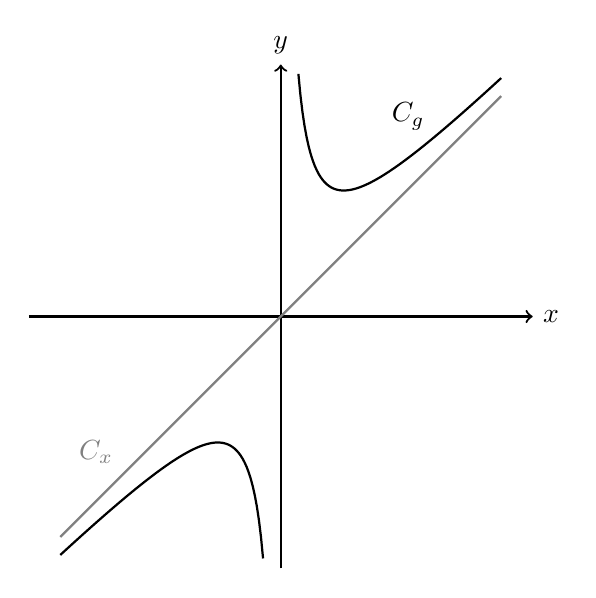
\begin{tikzpicture}[x=0.8cm, y=0.8cm, thick]

  % Axes
  \draw[->] (-4,0) -- (4,0) node[right] {\(x\)};
  \draw[->] (0,-4) -- (0,4) node[above] {\(y\)};

  % Asymptote y = x (gray)
  \draw[gray, thick, domain=-3.5:3.5] plot (\x, \x);
  \node[gray, above left] at (-2.5, -2.5) {\(C_x\)};

  % Function y = x + 1/x (black)
  \draw[black, thick, domain=-3.5:-0.28, samples=100] plot (\x, {\x + 1/\x});
  \draw[black, thick, domain=0.28:3.5, samples=100] plot (\x, {\x + 1/\x});
  
  % Labels
  \node[black, above right] at (1.6, 2.8) {\(C_g\)};

\end{tikzpicture}
\end{document}
